\documentclass[letterpaper,11pt,twoside,electronic,headers=exceptpdf,papers=countpages,linkcolor=blue]{confproc}

\renewcommand{\procpdfauthor}{Dennis Evangelista, Manalapan High School}
\renewcommand{\procpdftitle}{Journal of Science \& Engineering}
\renewcommand{\procchead}{}
\renewcommand{\proclhead}{}
\renewcommand{\proccfoot}{\thepage}

\author{\procpdfauthor}
\title{\procpdftitle}
\date{\today}
\renewcommand{\PAPERPATH}{.}

\makeindex

\usepackage{pdfpages}
\usepackage{helvet,mathptmx}
\renewcommand{\contentsname}{{\normalfont\sffamily Journal of\medskip}\\{\normalfont\Huge Science \& Engineering}}
\usepackage{verse}

\begin{document}
\frontmatter
\setcounter{page}{1}
\pdfbookmark[0]{Preamble}{preamble}
\pdfbookmark[1]{Cover}{cover}
%\maketitle
\index{Kilaru, Rishith}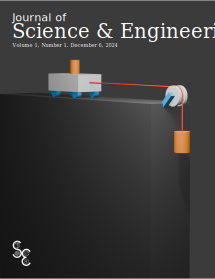
\includepdf[pages=1]{cover}
\newpage
Journal of Science Engineering (J S\&E) publishes high quality original research by promising students of science and engineering. 

% masthead here
Editorial staff

Editorial office

Advisory board

\vfill

Copytright \copyright\ 2024 The Journal of Science and Engineering.

Published by the {\scshape Freehold Regional High School District Press}.

s and e url here

This work is licensed under CC BY-NC 4.0. To view a copy of this license, visit \url{https://creativecommons.org/licenses/by-nc/4.0/}

library of congress titlepage information here


\otherpagestyle
\addtocontents{toc}{Volume 1, Number 1, \today\bigskip\\}
% The following hack is necessary to get Inside JS&E to be on back page 
\begingroup
\let\cleardoublepage=\clearpage
\tableofcontents
\addtocontents{toc}{\emph{From the cover:} Newton's second law relates force, mass, and acceleration and is often written as $\sum\vec{F}=m\vec{a}$. In this special issue of Journal of Science \& Engineering, researchers considered the validity of Newton's second law. \emph{Cover image: Rishith Kilaru.}\bigskip\\}
%Inside J S\&E here
%\section*{Inside J S\&E}
%\addcontentsline{toc}{section}{Inside J S\& E}
\vspace*{\fill}
\begin{verse}
String pulls cart down track\\
Weight provides a downward force\\
$\vec{F}$ equals $m$ $\vec{a}$
\end{verse}
\vspace{2ex}\raggedleft{Miguel Arenas, Callie Butash, Jake Chin, Kriti Malhotra,\\Grace Nealon, and Petra Rofman}\par
\index{Arenas, Miguel}\index{Butash, Callie}\index{Chin, Jake}\index{Malhotra, Kriti}\index{Nealon, Grace}\index{Rofman, Petra}
\vspace*{\fill}
\endgroup

\mainmatter
\procpaper[%
title={Testing Newton's second law in an accelerating system},
author={Miguel Arenas, Callie Butash, Jake Chin, Kriti Malhotra, Grace Nealon, and Petra Rofman},
index={\index{Arenas, Miguel}\index{Butash, Callie}\index{Chin, Jake}\index{Malhotra, Kriti}\index{Nealon, Grace}\index{Rofman, Petra}},
]{/arenas/arenas}

\procpaper[%
title={Verifying Newton's second law: the relationship between force and acceleration},
author={Dia Avalur, Srilekha Dantu, Jophy Lin, and Anika Tokala},
index={\index{Avalur, Dia}\index{Dantu, Srilekha}\index{Lin, Jophy}\index{Tokala, Anika}},
]{/avalur/avalur}

\procpaper[%
title={Investigating Newton's first law in a pulley system},
author={Andrew Barone, Alexander Gut, Rishith Kilaru, and Shrikar Swami},
index={\index{Barone, Andrew}\index{Gut, Alexander}\index{Kilaru, Rishith}\index{Swami, Shrikar}},
]{/barone/barone}

\procpaper[%
title={Experimental support for Newton's second law},
author={Cole Canada, Stefano D'Agostino, Ethan Fuks, Jason Katz, Ryan Leung, and Edmund Lee},
index={\index{Canada, Cole}\index{D'Agostino, Stefano}\index{Fuks, Ethan}\index{Katz, Jason}\index{Leung, Ryan}\index{Lee, Edmund}},
]{/canada/canada}

\procpaper[%
title={Newton's second law as demonstrated in a cart-pulley-mass system},
author={Vasudevan Govardhanen, Gage Grant, Aidan Dumalagan, Tushaar Akula, Daivik Jajoo, Rohan Avalur, Adrit Sikdar, and Jake Cacciarelli},
index={\index{Govardhanen, Vasudevan}\index{Grant, Gage}\index{Dumalagan, Aidan}\index{Akula, Tushaar}\index{Jajoo, Daivik}\index{Avalur, Rohan}\index{Sikdar, Adrit}\index{Cacciarelli, Jake}},
]{/govardhanen/govardhanen}

\procpaper[%
title={Examining the relationship between the net force and acceleration in a pulley system},
author={Siddharth Kedharnath, Samay Prabhu, Daniel Altman, and Joel D'Souza},
index={\index{Kedharnath, Siddharth}\index{Prabhu, Samay}\index{Altman, Daniel}\index{D'Souza, Joel}},
]{/kedharnath/kedharnath}

\procpaper[%
title={Relationship between Newton’s second law and acceleration, mass, and force},
author={Nitika Kishore, Sameera Patil, Anton Lavrenov, and Connor Paskiewicz},
index={\index{Kishore, Nitika}\index{Patil, Sameera}\index{Lavrenov, Anton}\index{Paskiewicz, Connor}},
]{/kishore/kishore}

\procpaper[%
title={Testing Newton's second law with cart and mass},
author={Sharone Krasnopolsky, Timur Neyir, and Brady Gorelczenko},
index={\index{Krasnopolsky, Sharone}\index{Neyir, Timur}\index{Gorelczenko, Brady}},
]{/krasnopolsky/krasnopolsky}

\procpaper[%
title={Experimental investigation of Newton's second law using a two-mass pulley system},
author={Andrew Fox, Brandon Heller, Dev Parekh, Joshua Perle, and Clay Stevens},
index={\index{Fox, Andrew}\index{Heller, Brandon}\index{Parekh, Dev}\index{Perle, Joshua}\index{Stevens, Clay}},
]{/perle/perle}

\procpaper[%
title={Verifying $\sum\vec{F} = m\vec{a}$},
author={Sagarika Yagnyeshwaran, Emily Chen, Andrew Kabatsky, Aleksandra Guimaraes, Vijita Ayyangar, and Aryanna Cetrulo},
index={\index{Yagnyeshwaran, Sagarika}\index{Chen, Emily}\index{Kabatsky, Andrew}\index{Guimaraes, Aleksandra}\index{Ayyangar, Vijita}\index{Cetrulo, Aryanna}},
]{/yagnyeshwaran/yagnyeshwaran}

\backmatter
%\bibliographystyle{plain}
%\bibliography{\procbibfile}

\insertindex

% get on even page?!
%\includepdf[pages=1]{main-confproc-old.pdf}
\end{document}